% !TeX TS-program = txs:///duck
\documentclass{standalone}
\usepackage{tikzducks}

\begin{document}
	
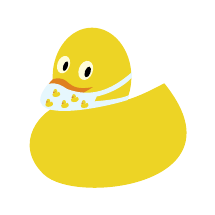
\begin{tikzpicture}
	\duck[]

  \begin{pgfinterruptboundingbox}
    \fill[cyan!10!white]  (1.4051,1.5586) .. controls (1.1370,1.3225) and (0.8775,1.2365) .. (0.5844,1.3462) .. controls (0.5190,1.3848) and (0.4601,1.4391) .. (0.3414,1.4100) .. controls (-0.1044,0.8610) and (1.0760,1.1140) .. (1.3547,1.2073) -- (1.3698,1.2679) .. controls (1.2783,1.2261) and (1.1035,1.2035) .. (0.9324,1.1895) -- (0.9600,1.2509) .. controls (1.1068,1.2809) and (1.2985,1.3700) .. (1.4071,1.4930) -- cycle;
  \end{pgfinterruptboundingbox}
  
  \duck[scale=0.05, shift={(6,22.3)}]
  \duck[scale=0.05, shift={(7.8,24.8)}]
  \duck[scale=0.05, shift={(10,22)}]
  \duck[scale=0.05, shift={(12.5,23.5)}]
  \duck[scale=0.05, shift={(15,22)}]  
  
\end{tikzpicture}	
	
\end{document}